% Τεχνική τεκμηρίωση του πακέτου αναλογικής απόσβεσης ανά κόμβο.
% Μεταγλώττιση από τον ριζικό κατάλογο:  xelatex DOCUMENTATION_GR.tex  (τρεις φορές, για τα περιεχόμενα)
\documentclass[11pt,a4paper]{article}
\usepackage[a4paper,top=2.5cm,bottom=2.5cm,left=2.2cm,right=2.2cm]{geometry}
\usepackage{amsmath,amsthm}
\usepackage{mathptmx}
\usepackage{amssymb}
\usepackage[no-math]{fontspec}
\usepackage[english,main=greek]{babel}
\babelfont{rm}[Language=Default,RawFeature={-ccmp}]{FreeSerif}
\babelfont{sf}[Language=Default,RawFeature={-ccmp}]{FreeSans}
\babelfont{tt}[Language=Default,Scale=0.86]{DejaVu Sans Mono}
\usepackage{microtype}
\usepackage{booktabs}
\usepackage{array}
\usepackage{longtable}
\usepackage[font=small,labelfont=bf,skip=4pt]{caption}
\usepackage{enumitem}
\setlist{itemsep=2pt,topsep=3pt}
\usepackage{tikz}
\usetikzlibrary{arrows.meta,positioning}
\usepackage{xurl}
\usepackage{xr-hyper}
\externaldocument[P-]{paper/paper_gr}  % αριθμοί πινάκων, σχημάτων και ενοτήτων της εργασίας (μεταγλωττίστε πρώτα την εργασία)
\usepackage[hidelinks]{hyperref}
\usepackage{placeins}
\emergencystretch=2em

\newtheorem{theorem}{Θεώρημα}
\newtheorem{lemma}{Λήμμα}
\newtheorem{corollary}{Πόρισμα}
\theoremstyle{definition}
\newtheorem{remark}{Παρατήρηση}
\theoremstyle{plain}
\newcommand{\genpropname}{}
\newtheorem*{genprop}{\genpropname}
\newenvironment{prop}[1]{\renewcommand{\genpropname}{Πρόταση #1}\begin{genprop}}{\end{genprop}}

\newcommand{\Pesc}{P_{\mathrm{esc}}}
\newcommand{\Pescbar}{\bar{P}_{\mathrm{esc}}}
\newcommand{\clip}{\mathrm{clip}}
\newcommand{\diag}{\mathrm{diag}}
\newcommand{\E}{\mathbb{E}}
\newcommand{\N}{\mathcal{N}}
\newcommand{\AP}{\mathrm{AP}}
\newcommand{\one}{\mathbf{1}}
\newcommand{\file}[1]{\path{#1}}

\input{paper/generated/macros.tex}
\input{paper/generated/tables_gr.tex}

\title{\textbf{Αυτοσυνεπής Αναλογική Απόσβεση ανά Κόμβο για την Κατάταξη Προσβασιμότητας σε Στοχαστικά Γραφήματα}\\[4pt]
\large Τεχνική τεκμηρίωση: αρχιτεκτονική, αποδείξεις, περιγραφή κώδικα, πολυπλοκότητα και οδηγός αναπαραγωγής}
\author{Ιωάννης Κωνσταντέλλος\\[2pt]
\small Τμήμα Μηχανικών Ηλεκτρονικών Υπολογιστών και Πληροφορικής\\
\small Πανεπιστήμιο Πατρών}
\date{Οκτώβριος 2026}

\begin{document}
\maketitle

\begin{abstract}
\noindent Το παρόν κείμενο συνοδεύει την εργασία \emph{«Αυτοσυνεπής Αναλογική Απόσβεση ανά Κόμβο για την Κατάταξη Προσβασιμότητας σε Στοχαστικά Γραφήματα: Ακριβής Θεωρία, Δυναμικά Εμπόδια και Υβριδική Εξομάλυνση Διπλού Τελεστή»} και την αγγλική της εκδοχή. Περιγράφει την αρχιτεκτονική του πακέτου λογισμικού που παρήγαγε κάθε αριθμό της εργασίας, δίνει πλήρεις αποδείξεις του Θεωρήματος~1 και των Προτάσεων~A--F και~$2'$ μαζί με τα βοηθητικά λήμματα στα οποία στηρίζεται η υλοποίηση, περιγράφει κάθε άρθρωμα του κώδικα, αναλύει τη χρονική και χωρική πολυπλοκότητα κάθε συνιστώσας και δίνει αναλυτικό οδηγό για την αναπαραγωγή των πειραμάτων, των πινάκων, των σχημάτων και των τεσσάρων εγγράφων PDF από την αρχή.
\end{abstract}

\tableofcontents

\section{Αντικείμενο και συμβάσεις}\label{sec:scope}

Το πακέτο μελετά την Αρχή της Αναλογικής Σχετικής Επιρροής για την απόσβεση ανά κορυφή στην κατάταξη προσβασιμότητας με διάχυση. Περιέχει (i)~μια διανυσματοποιημένη βιβλιοθήκη που υλοποιεί στιγμιότυπα στοχαστικών γραφημάτων, πραγματική τιμή αναφοράς Monte Carlo, τελεστές διάδοσης, αποσβεννύμενες διαχύσεις, μετάδοση μηνυμάτων, τις τρεις υλοποιήσεις της αρχής, την αγκυρωμένη οικογένεια δυνάμεων, την εξομάλυνση της Εκδοχής~(β), τα μαντεία και τις μετρικές· (ii)~τα προγράμματα εκτέλεσης μιας προκαταχωρισμένης αξιολόγησης σε \NTotal{} στιγμιότυπα· (iii)~προγράμματα ανάλυσης, ελέγχων και χρονομέτρησης· και (iv)~τις γεννήτριες κάθε μακροεντολής, πίνακα και σχήματος της εργασίας.

Ο συμβολισμός ακολουθεί την εργασία. Το $G=(V,E,p)$ είναι ένα μη κατευθυνόμενο στοχαστικό γράφημα με $n=|V|$ κορυφές και $m=|E|$ ακμές, καθεμία από τις οποίες υπάρχει ανεξάρτητα με πιθανότητα $p_{ij}\in(0,1]$· το $x>0$ με $\sum_ix_i=1$ είναι η αρχική κατανομή (prior)· το $y^*_i=\E\big[\sum_{v\in C(i)}x_v\big]$ είναι η αναμενόμενη προσβάσιμη μάζα. Τα διανύσματα συγκρίνονται κατά συνιστώσα, το $\circ$ είναι το γινόμενο κατά συνιστώσα, $\N(v)=v/\one^{\top}v$ και $\one$ το διάνυσμα με όλα τα στοιχεία ίσα με τη μονάδα. Στα ονόματα αρχείων, το \file{<panel>} είναι ένα από τα \texttt{dev}, \texttt{test}, \texttt{prior}, \texttt{real}, \texttt{scale}. Στα αρχεία αποτελεσμάτων, ο αριθμός βημάτων $T=10^6$ σημαίνει «εκτέλεση έως το σταθερό σημείο» ($T=\infty$).

\section{Αρχιτεκτονική}\label{sec:architecture}

\subsection{Οργάνωση του αποθετηρίου}

Ο Πίνακας~\ref{tab:layout} απαριθμεί τα αρχεία και τους καταλόγους του πακέτου.

\begin{longtable}{>{\raggedright\arraybackslash}p{5.3cm}>{\raggedright\arraybackslash}p{10.3cm}}
\caption{Οργάνωση του αποθετηρίου.}\label{tab:layout}\\
\toprule
Διαδρομή & Περιεχόμενο \\
\midrule
\endfirsthead
\caption[]{Οργάνωση του αποθετηρίου (συνέχεια).}\\
\toprule
Διαδρομή & Περιεχόμενο \\
\midrule
\endhead
\file{prop_damping_lib.py} & Η βιβλιοθήκη: στιγμιότυπα, αρχικές κατανομές, φόρτωση πραγματικών δικτύων, τελεστές, πραγματική τιμή αναφοράς Monte Carlo και ακριβής, μετρικές, διαχύσεις, μετάδοση μηνυμάτων, υλοποιήσεις, αγκυρωμένος νόμος, εξομάλυνση, μαντεία. \\
\file{build_panels.py} & Παράγει τα πέντε σύνολα στιγμιοτύπων και τα δύο ανεξάρτητα δείγματα πραγματικής τιμής αναφοράς τους. \\
\file{experiments.py} & Το στάδιο \texttt{grid} (πλήρης αναζήτηση στα σύνολα ανάπτυξης και ελέγχου) και το στάδιο \texttt{confirm} (αναφορές, μαντεία και παγωμένες διαμορφώσεις στα ανεξάρτητα σύνολα). \\
\file{select_configs.py} & Εξάγει εκ νέου τις παγωμένες διαμορφώσεις από τα αποτελέσματα ανάπτυξης με τους δηλωμένους κανόνες και επαληθεύει το \file{results/selected.json}. \\
\file{analysis.py} & Φόρτωση αποτελεσμάτων σταδίων, μέσοι όροι διαμορφώσεων, στατιστική κατά ζεύγη, διόρθωση Holm. \\
\file{controls.py}, \file{mf_controls.py} & Αντιστοιχισμένοι έλεγχοι: σταθερή απόσβεση, μέση τιμή ανά βήμα (δίδυμο μέσης τιμής) και μετάθεση του νόμου ανά κόμβο. \\
\file{sign_condition.py}, \file{prop2_stats.py} & Διαγνωστικά για την Πρόταση~E (συνθήκη προσήμου) και την Πρόταση~2 (ομοιομορφία αρχικής κατανομής). \\
\file{explore_rawP.py} & Διερευνητική (μη προκαταχωρισμένη) διάδοση στον ακατέργαστο $P$. \\
\file{mc_baseline.py}, \file{bench_runtime.py} & Αναφορές Monte Carlo με $k\in\{50,200,1000\}$ κόσμους και χρονομετρήσεις σε μία διεργασία. \\
\file{paper_extras.py} & Ίχνη δυναμικής, συμπληρωματικότητα τελεστών και σάρωση μεγέθους. \\
\file{make_checkpoint_tables.py}, \file{write_checkpoint_report.py} & Οι πίνακες και η αναφορά του πρώτου σημείου ελέγχου. \\
\file{make_paper_assets.py}, \file{paper_figures.py} & Κάθε μακροεντολή, πίνακας και σχήμα της εργασίας (αγγλικά και ελληνικά). \\
\file{tests/} & Θεμελιώδεις και δυναμικοί έλεγχοι (Θεώρημα~1, πραγματική τιμή αναφοράς, προτάσεις). \\
\file{data/<panel>/NNNN.npz} & Στιγμιότυπα με την πραγματική τιμή αναφοράς τους· το \file{data/<panel>/specs.json} απαριθμεί τις προδιαγραφές. \\
\file{results/} & Αποτελέσματα ανά στιγμιότυπο, έλεγχοι, διαγνωστικά, χρονομετρήσεις, η παγωμένη επιλογή και η σύνοψή της. \\
\file{paper/} & \file{paper_en.tex}, \file{paper_gr.tex}, τα παραγόμενα αρχεία στο \file{paper/generated/} και τα μεταγλωττισμένα PDF. \\
\file{figures/}, \file{figures_gr/} & Τα πέντε σχήματα με αγγλικές και ελληνικές ετικέτες. \\
\file{logs/} & Αρχεία προόδου των μακρών σταδίων (από αυτά προέρχονται οι χρόνοι εκτέλεσης που αναφέρονται εδώ). \\
\bottomrule
\end{longtable}

\subsection{Ροή δεδομένων}

Το Σχήμα~\ref{fig:pipeline} παρουσιάζει τη ροή επεξεργασίας. Κάθε στάδιο διαβάζει μόνο τις εξόδους προηγούμενων σταδίων, οπότε οποιοδήποτε στάδιο μπορεί να εκτελεστεί ξανά μεμονωμένα. Η επιλογή χρησιμοποιεί μόνο το σύνολο ανάπτυξης, και κάθε στάδιο ανεξάρτητης αξιολόγησης διαβάζει το αρχείο των παγωμένων διαμορφώσεων.

\begin{figure}[!ht]
\centering
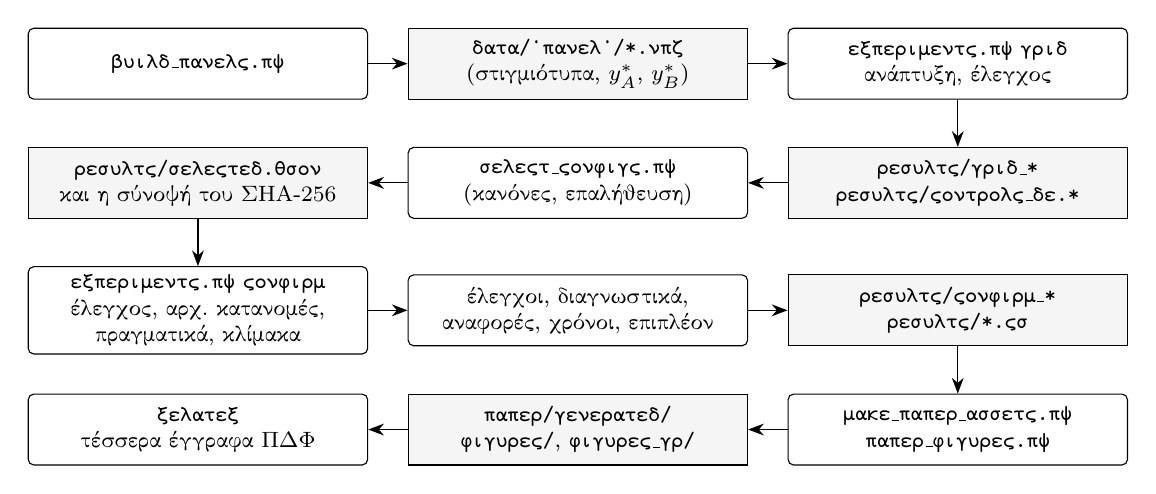
\begin{tikzpicture}[node distance=6mm and 5mm, font=\footnotesize,
  box/.style={draw, rounded corners=2pt, align=center, inner sep=3pt, minimum height=9mm, text width=4.1cm},
  data/.style={draw, align=center, inner sep=3pt, minimum height=9mm, text width=4.1cm, fill=black!4},
  arr/.style={-{Stealth[length=2mm]}}]
\node[box] (build) {\texttt{build\_panels.py}};
\node[data, right=of build] (data) {\texttt{data/<panel>/*.npz}\\(στιγμιότυπα, $y^*_A$, $y^*_B$)};
\node[box, right=of data] (grid) {\texttt{experiments.py grid}\\ανάπτυξη, έλεγχος};
\node[data, below=of grid] (gres) {\texttt{results/grid\_*}\\\texttt{results/controls\_dev.*}};
\node[box, left=of gres] (sel) {\texttt{select\_configs.py}\\(κανόνες, επαλήθευση)};
\node[data, left=of sel] (frozen) {\texttt{results/selected.json}\\και η σύνοψή του SHA-256};
\node[box, below=of frozen] (conf) {\texttt{experiments.py confirm}\\έλεγχος, αρχ.\ κατανομές,\\πραγματικά, κλίμακα};
\node[box, right=of conf] (aux) {έλεγχοι, διαγνωστικά,\\αναφορές, χρόνοι, επιπλέον};
\node[data, right=of aux] (res) {\texttt{results/confirm\_*}\\\texttt{results/*.csv}};
\node[box, below=of res] (assets) {\texttt{make\_paper\_assets.py}\\\texttt{paper\_figures.py}};
\node[data, left=of assets] (gen) {\texttt{paper/generated/}\\\texttt{figures/}, \texttt{figures\_gr/}};
\node[box, left=of gen] (tex) {\texttt{xelatex}\\τέσσερα έγγραφα PDF};
\draw[arr] (build) -- (data);
\draw[arr] (data) -- (grid);
\draw[arr] (grid) -- (gres);
\draw[arr] (gres) -- (sel);
\draw[arr] (sel) -- (frozen);
\draw[arr] (frozen) -- (conf);
\draw[arr] (conf) -- (aux);
\draw[arr] (aux) -- (res);
\draw[arr] (res) -- (assets);
\draw[arr] (assets) -- (gen);
\draw[arr] (gen) -- (tex);
\end{tikzpicture}
\caption{Ροή δεδομένων του πακέτου. Τα γκρίζα πλαίσια είναι αρχεία· τα λευκά είναι προγράμματα.}
\label{fig:pipeline}
\end{figure}

\subsection{Ντετερμινισμός}

Κάθε τυχαία επιλογή λαμβάνει σπόρο (seed) από τη συνάρτηση \texttt{stable\_seed(*parts)}, δηλαδή τα πρώτα 63 bit της σύνοψης SHA-256 του ρόλου της επιλογής (για παράδειγμα, το σύνολο, η οικογένεια, το μέγεθος, το εύρος πιθανοτήτων και η επανάληψη ενός στιγμιοτύπου, ή το όνομα του στιγμιοτύπου και ο σκοπός ενός δείγματος Monte Carlo). Επομένως οι σπόροι δεν εξαρτώνται από τη σειρά εκτέλεσης ούτε από τον αριθμό των διεργασιών, και η επανεκτέλεση οποιουδήποτε σταδίου αναπαράγει τα αποθηκευμένα αποτελέσματα ακριβώς, στην ίδια πλατφόρμα. Η τοπολογία και οι πιθανότητες ακμών ενός συνθετικού στιγμιοτύπου λαμβάνουν σπόρο ανεξάρτητα από την αρχική του κατανομή, και αυτό επιτρέπει στο σύνολο αρχικών κατανομών να μεταβάλλει μόνο την αρχική κατανομή.

\subsection{Μορφές αρχείων}

\paragraph{Στιγμιότυπα.} Το \file{data/<panel>/NNNN.npz} αποθηκεύει τα \texttt{edges} (ακέραιος πίνακας $m\times2$ με $i<j$), \texttt{p} (πιθανότητες ακμών), \texttt{x} (αρχική κατανομή), \texttt{yA} και \texttt{yB} (δύο ανεξάρτητες εκτιμήσεις της πραγματικής τιμής αναφοράς από \MGTsp{} κόσμους η καθεμία), \texttt{yA2} (η δεύτερη ροπή του δείγματος αξιολόγησης) και \texttt{meta} (συμβολοσειρά JSON με οικογένεια, μέγεθος, εύρος πιθανοτήτων, αρχική κατανομή, επανάληψη, $\Pescbar$, στατιστικά της αρχικής κατανομής και την αναφορά διαιρεμένου δείγματος). Η \texttt{load\_instance} επιστρέφει το στιγμιότυπο, τα \texttt{yA}, \texttt{yB} και τα μεταδεδομένα.

\paragraph{Αποτελέσματα.} Κάθε στάδιο γράφει το \file{results/<stage>_<panel>/<id>.csv.gz} με μία γραμμή ανά αξιολογούμενη μέθοδο ή διαμόρφωση και τις στήλες \texttt{id}, \texttt{method}, \texttt{T} (βήματα ή περάσματα· 0 για μεθόδους ενός βήματος), \texttt{beta} (βάρος συνδυασμού), \texttt{blend} (\texttt{s} συνδυασμός βαθμολογιών, \texttt{r} συνδυασμός τάξεων, \texttt{-} κανένας) και \texttt{rho} ($\rho$ του Spearman ως προς το $y^*_A$), καθώς και ένα αρχείο JSON με διαγνωστικά (προσαρμογές μαντείων, δυναμική, δευτερεύουσες μετρικές).

\paragraph{Ονόματα μεθόδων.} Το πρόθεμα του ονόματος μιας μεθόδου δηλώνει την οικογένειά της· τα πεδία μετά την άνω και κάτω τελεία χωρίζονται με κάθετες γραμμές.
\begin{center}\small
\begin{tabular}{>{\raggedright\arraybackslash}p{6.0cm}>{\raggedright\arraybackslash}p{9.4cm}}
\toprule
Πρόθεμα ή μοτίβο & Σημασία \\
\midrule
\texttt{base:} & διαχύσεις αναφοράς: \texttt{rule\_EW}, \texttt{fixed085}, \texttt{rule\_WT}, \texttt{local\_pesc} \\
\texttt{ref:} & αναφορές: \texttt{prior}, \texttt{Pesc}, \texttt{MP2}, \texttt{MPinf}, \texttt{ceiling} \\
\texttt{oracle:} & μαντεία: \texttt{scalar}, \texttt{scalar\_in}, \texttt{scalar\_WT}, \texttt{pernode} \\
\texttt{true:} & οι νόμοι ανά κόμβο με το αληθές $y^*$: \texttt{prop}, \texttt{ap0.5}, \texttt{ap1.0} \\
\texttt{sa:kind|op|scale|gamma} & αυτόνομες υλοποιήσεις \\
\texttt{ap:eta} & ο αγκυρωμένος νόμος \\
\texttt{free:gamma|eta} & ο μη αγκυρωμένος νόμος \\
\texttt{pb:base|eta|mode} & αγκυρωμένη εξομάλυνση (\texttt{fix}: σταθερό $\alpha$· \texttt{sc}: αυτοσυνεπής) \\
\texttt{pbx:base|kind|op|scale|gamma} & εξομάλυνση με υλοποίηση \\
\texttt{pbperm:base} & αγκυρωμένη εξομάλυνση με μετάθεση \\
\texttt{sel:NAME} & μια παγωμένη διαμόρφωση \\
\bottomrule
\end{tabular}
\end{center}

\paragraph{Παγωμένες διαμορφώσεις.} Το \file{results/selected.json} αντιστοιχίζει καθένα από τα \NFrozen{} ονόματα στις παραμέτρους του (Πίνακας~\ref{tab:configs})· το \file{results/selected.sha256} καταγράφει τη σύνοψή του (που αρχίζει με \texttt{\SelHash}) και τη στιγμή του παγώματος (\SelTime).

\TabConfigs

\section{Μαθηματικά θεμέλια}\label{sec:math}

Η ενότητα αυτή συγκεντρώνει κάθε μαθηματική πρόταση που χρησιμοποιείται από την εργασία ή από την υλοποίηση, με πλήρεις αποδείξεις. Σε όλη την ενότητα $T\ge0$ κατά στοιχείο· ο $T$ είναι \emph{υποστοχαστικός κατά γραμμές} αν $T\one\le\one$· με $\rho(\cdot)$ συμβολίζεται η φασματική ακτίνα.

\subsection{Βοηθητικά αποτελέσματα που χρησιμοποιεί η υλοποίηση}

\begin{lemma}[κανονικοποιημένη αποσβεννύμενη διάχυση]\label{lem:diffusion}
Έστω $\alpha\in[0,1]^n$, $D=\diag(\alpha)$ και $B(\alpha)=(I-D)\,x\,\one^{\top}+DT$. Ένα διάνυσμα $y>0$ με $\one^{\top}y=1$ είναι σταθερό σημείο της $y\mapsto\N\big((1-\alpha)\circ x+\alpha\circ Ty\big)$ αν και μόνο αν είναι ιδιοδιάνυσμα του $B(\alpha)$ με ιδιοτιμή $\lambda=\one^{\top}B(\alpha)y>0$· τότε ικανοποιεί $\lambda y=(I-D)x+DTy$. Αν $\alpha_i<1$ για κάθε $i$, τότε $B(\alpha)>0$ κατά στοιχείο, το ιδιοδιάνυσμα είναι μοναδικό (το διάνυσμα Perron), και τόσο η απλή όσο και η οκνηρή μέθοδος δυνάμεων συγκλίνουν σε αυτό από κάθε θετική εκκίνηση. Αν ο $B(\alpha)$ είναι απλώς μη αναγώγιμος (για παράδειγμα $\alpha\equiv1$ και $T$ μη αναγώγιμος αλλά περιοδικός), η οκνηρή επανάληψη $y\leftarrow\N\big(\tfrac12(y+B(\alpha)y)\big)$ εξακολουθεί να συγκλίνει στο διάνυσμα Perron.
\end{lemma}

\begin{proof}
Για $\one^{\top}y=1$ ισχύει $B(\alpha)y=(I-D)x+DTy$, οπότε η εξίσωση σταθερού σημείου $y=\N(B(\alpha)y)$ γράφεται $B(\alpha)y=(\one^{\top}B(\alpha)y)\,y$. Αν κάθε $\alpha_i<1$, ο όρος τάξης ένα $(I-D)x\one^{\top}$ είναι θετικός κατά στοιχείο, άρα $B(\alpha)>0$, και το θεώρημα του Perron~\cite{hornjohnson13} δίνει απλή, γνησίως κυρίαρχη ιδιοτιμή με θετικό ιδιοδιάνυσμα, το μόνο θετικό ιδιοδιάνυσμα με ακρίβεια κλίμακας· η μέθοδος δυνάμεων συγκλίνει σε αυτό από κάθε θετική εκκίνηση. Ο οκνηρός πίνακας $\tfrac12(I+B)$ έχει τα ίδια ιδιοδιανύσματα και ιδιοτιμές $\tfrac12(1+\mu)$. Αν ο $B$ είναι μη αναγώγιμος με ρίζα Perron $r$, κάθε άλλη ιδιοτιμή ικανοποιεί $|\tfrac12(1+\mu)|\le\tfrac12(1+|\mu|)\le\tfrac12(1+r)$, με ισότητα μόνο όταν $\mu=r$· επομένως η $\tfrac12(1+r)$ είναι γνησίως κυρίαρχη, και η οκνηρή μέθοδος δυνάμεων συγκλίνει ακόμη κι όταν ο $B$ έχει άλλες ιδιοτιμές μέτρου $r$ (περιοδική περίπτωση).
\end{proof}

\begin{lemma}[σταθερά αγκύρωσης]\label{lem:anchor}
Για πραγματικούς αριθμούς $\ell_1,\dots,\ell_n$ και $\alpha_0\in(0,1)$ υπάρχει μοναδικό $c\in\mathbb R$ με $\frac1n\sum_i\sigma(c+\ell_i)=\alpha_0$, όπου $\sigma$ η λογιστική συνάρτηση. Μια επανάληψη Newton, προστατευμένη από το διάστημα $[\mathrm{logit}(\alpha_{\min})-\max|\ell|-1,\ \mathrm{logit}(\alpha_{\max})+\max|\ell|+1]$ και από διχοτόμηση, συγκλίνει σε αυτό.
\end{lemma}

\begin{proof}
Η $h(c)=\frac1n\sum_i\sigma(c+\ell_i)$ είναι συνεχής και γνησίως αύξουσα, με $h(c)\to0$ όταν $c\to-\infty$ και $h(c)\to1$ όταν $c\to\infty$, οπότε η $h(c)=\alpha_0$ έχει ακριβώς μία λύση, η οποία ανήκει στο διάστημα επειδή στα άκρα του η $h$ είναι κάτω από $\alpha_{\min}\le\alpha_0$ και πάνω από $\alpha_{\max}\ge\alpha_0$. Η υλοποίηση ενημερώνει το διάστημα με βάση το πρόσημο του $h(c)-\alpha_0$ και αντικαθιστά κάθε βήμα Newton που βγαίνει έξω από αυτό με το μέσο του, οπότε το διάστημα συρρικνώνεται σε κάθε διχοτόμηση· η $h$ είναι λεία, και η μέθοδος Newton συγκλίνει τοπικά τετραγωνικά.
\end{proof}

\begin{lemma}[Monte Carlo κατά δέσμες]\label{lem:mc}
Έστω $G'_1,\dots,G'_b$ ανεξάρτητοι κόσμοι και $H$ η ξένη ένωσή τους, δηλαδή το γράφημα $b\,n$ κορυφών του οποίου το μπλοκ $w$ περιέχει τις ακμές του $G'_w$. Οι συνεκτικές συνιστώσες του $H$ είναι ακριβώς οι συνιστώσες των μεμονωμένων κόσμων. Συνεπώς ο εκτιμητής $\hat y_i=\frac1M\sum_{w=1}^M\sum_{v\in C_w(i)}x_v$, υπολογιζόμενος ανά δέσμη, είναι αμερόληπτος για το $y^*_i$ με διασπορά $\mathrm{Var}\big(\sum_{v\in C(i)}x_v\big)/M$, την οποία εκτιμά η δεύτερη ροπή που αποθηκεύεται στο \texttt{yA2}.
\end{lemma}

\begin{proof}
Το $H$ δεν έχει ακμές μεταξύ διαφορετικών μπλοκ, οπότε κάθε μονοπάτι, άρα και κάθε συνιστώσα, βρίσκεται μέσα σε ένα μπλοκ, όπου ταυτίζεται με μια συνιστώσα του αντίστοιχου κόσμου. Οι προσθετέοι $\sum_{v\in C_w(i)}x_v$ είναι ανεξάρτητα αντίγραφα του $\sum_{v\in C(i)}x_v$· η γραμμικότητα της αναμενόμενης τιμής και η ανεξαρτησία δίνουν τη μέση τιμή και τη διασπορά.
\end{proof}

\begin{lemma}[μετάδοση μηνυμάτων με μηδέν επαναλήψεις]\label{lem:knz}
Στη μορφή συμμετοχής της μετάδοσης μηνυμάτων του~\cite{knz14}, με όλα τα μηνύματα αρχικά ίσα με τη μονάδα, η συμμετοχή της κορυφής μετά από μηδέν επαναλήψεις είναι $\mu_i=1-\prod_{j\in N(i)}(1-p_{ij})=\Pesc(i)$.
\end{lemma}

\begin{proof}
Η έξοδος της κορυφής είναι $\mu_i=1-\prod_{j\in N(i)}(1-p_{ij}\nu_{j\to i})$, και με $\nu\equiv1$ αυτή είναι η πιθανότητα διαφυγής. Η υλοποίηση υπολογίζει το γινόμενο σε λογαριθμικό χώρο,
\[
\mu_i=-\mathrm{expm1}\Big(\sum_j\log1p(-p_{ij}\nu_{j\to i})\Big),
\]
που συμφωνεί με το $\Pesc$ με απόκλιση έως \KNZzeroDiff{} στους ελέγχους.
\end{proof}

\begin{lemma}[εμφύτευση περίσσειας]\label{lem:embed}
Για $y^{\mathrm{base}}>0$ και $\gamma>0$ έστω $z=\N(y^{\mathrm{base}})/\big(\tfrac1n\sum_j\N(y^{\mathrm{base}})_j/x_j\big)$ και $y^{(0)}=x+\gamma z$. Τότε $y^{(0)}>x$, οι λόγοι περίσσειας $(y^{(0)}_i-x_i)/x_i$ έχουν μέση τιμή ακριβώς $\gamma$, και η κατάταξη της περίσσειας $y^{(0)}-x$ ταυτίζεται με εκείνη του $y^{\mathrm{base}}/x$.
\end{lemma}

\begin{proof}
Εκ κατασκευής $z>0$ και $\frac1n\sum_iz_i/x_i=1$, άρα $\frac1n\sum_i(y^{(0)}_i-x_i)/x_i=\gamma$. Οι λόγοι περίσσειας $\gamma z_i/x_i$ είναι θετικό πολλαπλάσιο του $y^{\mathrm{base}}_i/x_i$.
\end{proof}

\subsection{Θεώρημα 1}

\begin{theorem}[ακριβής λύση του συζευγμένου συστήματος]\label{thm:factor}
Έστω $x_i>0$ και $S_i\ge0$. Ένα ζεύγος $(y_i,\alpha_i)$ με $y_i>0$ και $\alpha_i\ne1$ λύνει το
\[
y_i=(1-\alpha_i)x_i+\alpha_iS_i,\qquad \frac{\alpha_i}{1-\alpha_i}=\frac{y_i-x_i}{x_i}
\]
αν και μόνο αν $\alpha_i=1-x_i/y_i$ και $(y_i-x_i)(y_i+x_i-S_i)=0$. Οι λύσεις είναι ο τετριμμένος κλάδος $(x_i,0)$ και, όταν $S_i>x_i$, ο ενεργός κλάδος $y_i=S_i-x_i$, $\alpha_i=(S_i-2x_i)/(S_i-x_i)$, ο οποίος έχει $\alpha_i\in(0,1)$ αν και μόνο αν $S_i>2x_i$. Το τριώνυμο $y_i^2-S_iy_i+x_iS_i-x_i^2$ έχει διακρίνουσα $(S_i-2x_i)^2$, οπότε οι κλάδοι συναντώνται ακριβώς στο $S_i=2x_i$.
\end{theorem}

\begin{proof}
\emph{Βήμα 1.} Αν $\alpha_i\ne1$, η εξίσωση αναλογίας είναι ισοδύναμη με $\frac{\alpha_i}{1-\alpha_i}+1=\frac{y_i}{x_i}$, δηλαδή $\frac1{1-\alpha_i}=\frac{y_i}{x_i}$, δηλαδή $\alpha_i=1-\frac{x_i}{y_i}$ (χρησιμοποιώντας $y_i\ne0$). \emph{Βήμα 2.} Αντικαθιστώντας $1-\alpha_i=x_i/y_i$ και $\alpha_i=(y_i-x_i)/y_i$ στην εξίσωση διάχυσης και πολλαπλασιάζοντας με $y_i>0$ λαμβάνουμε την ισοδύναμη εξίσωση $y_i^2=x_i^2+(y_i-x_i)S_i$. \emph{Βήμα 3.} Με αναδιάταξη, $(y_i^2-x_i^2)-S_i(y_i-x_i)=0$, και η παραγοντοποίηση $y_i^2-x_i^2=(y_i-x_i)(y_i+x_i)$ δίνει $(y_i-x_i)(y_i+x_i-S_i)=0$. Σε ανεπτυγμένη μορφή, $y_i^2-S_iy_i+x_iS_i-x_i^2=0$, με διακρίνουσα $S_i^2-4(x_iS_i-x_i^2)=(S_i-2x_i)^2$ και ρίζες $\tfrac12\big(S_i\pm|S_i-2x_i|\big)$, δηλαδή $x_i$ και $S_i-x_i$. \emph{Βήμα 4.} Η ρίζα $y_i=x_i$ δίνει $\alpha_i=0$. Η ρίζα $y_i=S_i-x_i$ είναι αποδεκτή ($y_i>0$) αν και μόνο αν $S_i>x_i$, και τότε $\alpha_i=1-x_i/(S_i-x_i)=(S_i-2x_i)/(S_i-x_i)$· ο παρονομαστής είναι θετικός, άρα $\alpha_i>0$ αν και μόνο αν $S_i>2x_i$, και πάντοτε $\alpha_i<1$. \emph{Επαλήθευση.} Με $y_i=S_i-x_i$ και $\alpha_i=(S_i-2x_i)/(S_i-x_i)$: $(1-\alpha_i)x_i+\alpha_iS_i=\big(x_i^2+S_i^2-2x_iS_i\big)/(S_i-x_i)=S_i-x_i$, και $\alpha_i/(1-\alpha_i)=(S_i-2x_i)/x_i=(y_i-x_i)/x_i$.
\end{proof}

\begin{remark}[η κλίμακα του τελεστή]\label{rem:scale}
Στον στόχο, ο ενεργός κλάδος απαιτεί $S=Ty^*=y^*+x$. Αφού $y^*>0$ και $(Ty^*)_i/y^*_i=1+x_i/y^*_i>1$ για κάθε $i$, το φράγμα Collatz--Wielandt (Λήμμα~\ref{lem:cw}) δίνει $\rho(T)>1$. Επομένως κανένας τελεστής με $\rho(T)\le1$ --- ειδικότερα κανένας υποστοχαστικός κατά γραμμές τελεστής, όπως οι $W$ και $EW$ --- δεν μπορεί να ικανοποιεί το συζευγμένο σύστημα στον στόχο στον ενεργό κλάδο.
\end{remark}

\begin{lemma}[κάτω φράγμα Collatz--Wielandt~{\cite[Θεώρ.~8.1.26]{hornjohnson13}}]\label{lem:cw}
Αν $A\ge0$, $v>0$ και $Av\ge cv$ για πραγματικό $c$, τότε $\rho(A)\ge c$.
\end{lemma}

\subsection{Κατάρρευση, απορρόφηση και αστάθεια}

\begin{prop}{A}[κατάρρευση της Υλοποίησης Α σε πεπερασμένο χρόνο]
Έστω $T$ υποστοχαστικός κατά γραμμές, $x=\tfrac1n\one$, και $y^{(t+1)}=\max\big(x,Ty^{(t)}-x\big)$ με $y^{(0)}\ge x$. Τότε το $M_t=\max_iy_i^{(t)}$ ικανοποιεί $M_{t+1}\le\max\big(\tfrac1n,M_t-\tfrac1n\big)$ και $y^{(t)}=x$ για κάθε $t\ge\lceil nM_0\rceil-1$· από το $y^{(0)}=x+Tx$ η κατάρρευση συμβαίνει στο $t=1$.
\end{prop}

\begin{proof}
\emph{Αναλλοιώτητα.} $y^{(t)}\ge x$ για κάθε $t$: ισχύει για $t=0$ και διατηρείται από το μέγιστο. \emph{Συστολή του μεγίστου.} Αφού $T\ge0$, ισχύει $(Ty)_i\le\sum_jT_{ij}\max_ky_k\le M_t$, επειδή τα αθροίσματα γραμμών είναι το πολύ ένα. Επομένως $y_i^{(t+1)}=\max(\tfrac1n,(Ty^{(t)})_i-\tfrac1n)\le\max(\tfrac1n,M_t-\tfrac1n)$ για κάθε $i$. \emph{Επαγωγή.} $M_t\le\max(\tfrac1n,M_0-\tfrac tn)$· μόλις $t\ge nM_0-1$ το δεξί μέλος γίνεται $\tfrac1n$, και μαζί με το $y^{(t)}\ge x=\tfrac1n\one$ αυτό επιβάλλει $y^{(t)}=x$. \emph{Στασιμότητα.} Στο $y=x$ ισχύει $Tx\le x$ (αθροίσματα γραμμών το πολύ ένα), άρα $Tx-x\le0<x$ και η ενημέρωση επιστρέφει $x$. \emph{Θερμή εκκίνηση.} $y^{(0)}=x+Tx\le2x$, άρα $M_0\le2/n$ και $\lceil nM_0\rceil-1\le1$.
\end{proof}

\begin{prop}{B}[απορρόφηση και τετραγωνική συστολή της Υλοποίησης Β]
Έστω $T$ υποστοχαστικός κατά γραμμές και $y^{(t+1)}_i=(1-\alpha_i)x_i+\alpha_iS_i$ με $\alpha_i=e_i/(e_i+x_i)$, $e_i=(y_i^{(t)}-x_i)_+$ και $S=Ty^{(t)}$. (i)~Αν $y_i^{(t)}\le x_i$, τότε $y_i^{(s)}=x_i$ για κάθε $s>t$. (ii)~Αν $x=\xi\one$ και $m_t=\max_i(y_i^{(t)}-\xi)_+$, τότε $m_{t+1}\le m_t^2/(\xi+m_t)$· άρα $m_t\le m_0\,\theta^t$ με $\theta=m_0/(\xi+m_0)<1$, η σύγκλιση είναι τετραγωνική μόλις $m_t\ll\xi$, και $y^{(t)}\to x$.
\end{prop}

\begin{proof}
(i) Το $e_i=0$ δίνει $\alpha_i=0$ και $y_i^{(t+1)}=x_i$· τότε $e_i=0$ και στο επόμενο βήμα, κ.ο.κ. (ii) Η απεικόνιση $e\mapsto e/(e+\xi)$ είναι αύξουσα, άρα $\alpha_i\le m_t/(m_t+\xi)$. Κάθε $y_j^{(t)}\le\xi+m_t$, και ο $T$ είναι υποστοχαστικός κατά γραμμές και μη αρνητικός, άρα $S_i\le\xi+m_t$. Αν $S_i\le\xi$, το $y_i^{(t+1)}$ είναι κυρτός συνδυασμός των $\xi$ και $S_i\le\xi$ και δεν έχει περίσσεια. Διαφορετικά $y_i^{(t+1)}-\xi=\alpha_i(S_i-\xi)\le\frac{m_t}{m_t+\xi}\,m_t$. Το μέγιστο ως προς $i$ δίνει το φράγμα. Αφού $m_{t+1}\le m_t\cdot\frac{m_t}{\xi+m_t}\le m_t\,\theta$ (επειδή $m_t\le m_0$ και η $m\mapsto m/(\xi+m)$ είναι αύξουσα), η επαγωγή δίνει $m_t\le m_0\theta^t$· όταν $m_t\ll\xi$, $m_{t+1}\le m_t^2/\xi$. Οι κορυφές με $y^{(t)}_i<\xi$ επιστρέφουν στο $\xi$ στο επόμενο βήμα λόγω του~(i), άρα $y^{(t)}\to x$.
\end{proof}

\begin{prop}{C}[αστάθεια της αυτοσυνεπούς λύσης]
Έστω $T\ge0$ και $y>0$ με $y=Ty-x$ και $Ty>2x$. Τότε (i)~$\rho(T)>1$· (ii)~οι Ιακωβιανές των απεικονίσεων Α και Β στο $y$ είναι $J_A=T$ και $J_B=\diag(x/y)+\diag(\one-x/y)T$, αμφότερες μη αρνητικές με φασματική ακτίνα μεγαλύτερη της μονάδας· (iii)~για $T=\lambda W$ με $W$ στοχαστικό κατά γραμμές και $x=\xi\one$, το $y=x/(\lambda-1)$ είναι τέτοιο σημείο αν και μόνο αν $1<\lambda<2$, και τότε $\rho(J_A)=\lambda$ και $\rho(J_B)=-\lambda^2+3\lambda-1>1$.
\end{prop}

\begin{proof}
(i) $(Ty)_i/y_i=1+x_i/y_i\ge1+\min_jx_j/y_j>1$· εφαρμόζεται το Λήμμα~\ref{lem:cw}. (ii) Στο ενεργό σύνολο η απεικόνιση της Α είναι αφινική, $y\mapsto Ty-x$, με Ιακωβιανή $T$. Για τη Β γράφουμε $F_i(y)=x_i^2/y_i+(1-x_i/y_i)S_i(y)$ με $S=Ty$. Τότε $\partial F_i/\partial y_j=\delta_{ij}\big(-x_i^2/y_i^2+x_iS_i/y_i^2\big)+(1-x_i/y_i)T_{ij}$. Στο σταθερό σημείο $S_i=y_i+x_i$, οπότε ο διαγώνιος όρος είναι $x_i(S_i-x_i)/y_i^2=x_i/y_i$, γεγονός που δίνει την $J_B$. Επειδή $y=S-x>x$, τα $x/y$ και $\one-x/y$ είναι θετικά, άρα $J_B\ge0$. Επιπλέον $J_Ay=Ty=y+x>y$ και $J_By=x+(\one-x/y)\circ(y+x)=y+x\circ(y-x)/y>y$· το Λήμμα~\ref{lem:cw} δίνει $\rho(J_A)>1$ και $\rho(J_B)>1$. Ένα σταθερό σημείο απεικόνισης κλάσης $C^1$ της οποίας η Ιακωβιανή έχει ιδιοτιμή μέτρου μεγαλύτερου της μονάδας είναι ασταθές (αστάθεια μέσω γραμμικοποίησης). (iii) $W\one=\one$, άρα το $y=c\one$ λύνει την $y=\lambda Wy-\xi\one$ αν και μόνο αν $c(\lambda-1)=\xi$· η θετικότητα απαιτεί $\lambda>1$, και το $y>x$ (ισοδύναμα $Ty>2x$) απαιτεί $c>\xi$, δηλαδή $\lambda<2$. Τότε $x/y=(\lambda-1)\one$ και $J_B=(\lambda-1)I+(2-\lambda)\lambda W$. Για $a,b\ge0$ και μη αρνητικό $W$ με $\rho(W)=1$, οι ιδιοτιμές του $aI+bW$ είναι $a+b\mu$ με $|a+b\mu|\le a+b$, και το $a+b$ επιτυγχάνεται για $\mu=1$· άρα $\rho(J_B)=(\lambda-1)+(2-\lambda)\lambda=-\lambda^2+3\lambda-1$, και $\rho(J_B)-1=(\lambda-1)(2-\lambda)>0$ στο $(1,2)$. Επίσης $\rho(J_A)=\lambda\rho(W)=\lambda$.
\end{proof}

\subsection{Υλοποίηση Γ}

\begin{prop}{D}[συστολή μέσου Lehmer κάτω από την αρχική κατανομή]
Έστω $\gamma=1$, $T$ υποστοχαστικός κατά γραμμές, $f(x_i,s)=(x_i^2+s^2)/(x_i+s)$ και $y^{(0)}>0$. (i)~$f(x_i,s)\ge(2\sqrt2-2)x_i$, με ισότητα αν και μόνο αν $s=(\sqrt2-1)x_i$· η $f$ είναι φθίνουσα ως προς $s$ στο $[0,(\sqrt2-1)x_i]$ και αύξουσα στη συνέχεια· $f(x_i,s)<x_i$ αν και μόνο αν $0<s<x_i$. (ii)~Για $X\ge\max(\max_ix_i,\max_iy_i^{(0)})$ το υπερορθογώνιο $\mathcal B=\{(2\sqrt2-2)x\le y\le X\one\}$ περιέχει κάθε επανάληψη από το $t=1$, και η $F(y)_i=f(x_i,(Ty)_i)$ είναι συστολή στη νόρμα $\infty$ επί του $\mathcal B$, οπότε η επανάληψη συγκλίνει σε μοναδικό σταθερό σημείο $y^C$. (iii)~Στο $y^C$ ισχύει $y^C_i<x_i$ όποτε $0<S_i<x_i$, και μια απομονωμένη κορυφή κατατάσσεται πάνω από κάθε μη απομονωμένη κορυφή με την ίδια αρχική μάζα και $S_i<x_i$.
\end{prop}

\begin{proof}
(i) Με $r=s/x_i\ge0$, $\varphi(r)=f/x_i=(1+r^2)/(1+r)$ και $\varphi'(r)=(r^2+2r-1)/(1+r)^2$, της οποίας η μόνη μη αρνητική ρίζα είναι η $r^\star=\sqrt2-1$· $\varphi'<0$ στο $[0,r^\star)$ και $\varphi'>0$ μετά. $\varphi(r^\star)=(1+3-2\sqrt2)/\sqrt2=2\sqrt2-2$. Τέλος $f<x_i$ αν και μόνο αν $x_i^2+s^2<x_i^2+x_is$, δηλαδή $s(s-x_i)<0$, δηλαδή $0<s<x_i$.
(ii) \emph{Αναλλοιώτητα.} Από το (i), $y^{(t)}\ge(2\sqrt2-2)x$ για $t\ge1$. Ο μέσος Lehmer $L_2(a,b)=(a^2+b^2)/(a+b)$ βρίσκεται στο $[\min(a,b),\max(a,b)]$: αν $a\le b$, τότε $a(a+b)\le a^2+b^2\le b(a+b)$. Αφού ο $T$ είναι υποστοχαστικός κατά γραμμές, $S_i\le\max_jy_j^{(t)}$, άρα επαγωγικά $y^{(t+1)}_i\le\max(x_i,\max_jy_j^{(t)})\le X$. \emph{Συστολή.} $\partial F_i/\partial y_j=c_iT_{ij}$ με $c_i=\partial_sf(x_i,S_i)=1-2x_i^2/(x_i+S_i)^2$, που είναι αύξουσα ως προς $S_i$ και ανήκει στο $(-1,1)$ για $S_i>0$. Στο $\mathcal B$, μια κορυφή με γείτονα έχει $S_i\in[s_i^-,X]$ με $s_i^-=(2\sqrt2-2)(Tx)_i>0$, άρα $|c_i|\le\kappa_i=\max\big(|c(s_i^-)|,|c(X)|\big)<1$· μια απομονωμένη κορυφή έχει $T_{ij}=0$ για κάθε $j$. Επομένως $\|J_F(y)\|_\infty=\max_i|c_i|\sum_jT_{ij}\le\kappa=\max_i\kappa_i<1$ στο $\mathcal B$. Το $\mathcal B$ είναι κυρτό, οπότε η ανισότητα μέσης τιμής δίνει $\|F(y)-F(y')\|_\infty\le\kappa\|y-y'\|_\infty$, και το θεώρημα σταθερού σημείου του Banach δίνει μοναδικό σταθερό σημείο στο $\mathcal B$ που έλκει κάθε επανάληψη. Τα υπερορθογώνια είναι εμφωλευμένα ως προς $X$, άρα το σταθερό σημείο δεν εξαρτάται από το $X$ ούτε από την εκκίνηση. (iii) Εφαρμόζεται το (i) στο $y^C_i=f(x_i,S_i)$· μια απομονωμένη κορυφή έχει $S_i=0$ και $y^C_i=f(x_i,0)=x_i$.
\end{proof}

\subsection{Το εμπόδιο προσήμου}

\begin{lemma}[κυριαρχία της διαγωνίου στη στήλη]\label{lem:column}
Έστω $M\ge0$ υποστοχαστικός κατά γραμμές με $\rho(M)<1$ και $G=(I-M)^{-1}$. Τότε $G\ge0$ και $g_{jk}\le g_{kk}$ για κάθε $j,k$.
\end{lemma}

\begin{proof}
Η σειρά $G=\sum_{m\ge0}M^m\ge0$ συγκλίνει επειδή $\rho(M)<1$, και $g_{kk}\ge1$. Από την $G=I+MG$, η στήλη $v=Ge_k/g_{kk}$ ικανοποιεί $v_k=1$ και $v_j=\sum_lM_{jl}v_l$ για $j\ne k$. Έστω ότι $\mu=\max_jv_j>1$ και $A=\{j:v_j=\mu\}$, οπότε $k\notin A$. Για $j\in A$ ισχύει $\mu=\sum_lM_{jl}v_l\le\mu\sum_lM_{jl}\le\mu$· η ισότητα παντού επιβάλλει $\sum_lM_{jl}=1$ και $v_l=\mu$ όποτε $M_{jl}>0$, δηλαδή κάθε γραμμή με δείκτη στο $A$ αθροίζει στη μονάδα και έχει φορέα εντός του $A$. Τότε ο κύριος υποπίνακας $M_{AA}$ είναι στοχαστικός κατά γραμμές, άρα $\rho(M_{AA})=1$· όμως $\rho(M_{AA})\le\rho(M)<1$ για κύριο υποπίνακα μη αρνητικού πίνακα~\cite{hornjohnson13}, αντίφαση. Επομένως $v\le\one$.
\end{proof}

\begin{prop}{E}[εμπόδιο προσήμου]
(i)~Για $u_i=(1-\alpha_i)x_i+\alpha_iS_i$ ισχύει $\partial u_i/\partial\alpha_i=S_i-x_i$. (ii)~Έστω $T$ υποστοχαστικός κατά γραμμές, $\alpha\in[0,1)^n$, $D=\diag(\alpha)$, $y(\alpha)=(I-DT)^{-1}(I-D)x$ και $S=Ty$. Τότε $\partial y/\partial\alpha_k=(S_k-x_k)Ge_k$ με $G=(I-DT)^{-1}$, και η $\partial(y_k-y_j)/\partial\alpha_k=(S_k-x_k)(g_{kk}-g_{jk})$ έχει το πρόσημο του $S_k-x_k$ ή μηδενίζεται. (iii)~Για $T=EW$ και $x=\tfrac1n\one$, $(EWx)_i=\Pesc(i)/n<x_i$ όποτε $\Pesc(i)<1$.
\end{prop}

\begin{proof}
(i) Με παραγώγιση. (ii) Ο $DT$ είναι μη αρνητικός με αθροίσματα γραμμών το πολύ $\max_k\alpha_k<1$, άρα $\rho(DT)<1$, ο $I-DT$ είναι αντιστρέψιμος και το $y$ είναι καλά ορισμένο. Παραγωγίζοντας την $y=(I-D)x+DTy$ ως προς $\alpha_k$ λαμβάνουμε $\partial y=-x_ke_k+(Ty)_ke_k+DT\,\partial y$, δηλαδή $(I-DT)\partial y=(S_k-x_k)e_k$. Το Λήμμα~\ref{lem:column} με $M=DT$ δίνει $g_{kk}-g_{jk}\ge0$. (iii) Για μη απομονωμένη κορυφή $(W\one)_i=1$, άρα $(EW\tfrac1n\one)_i=\Pesc(i)/n$· μια απομονωμένη κορυφή έχει $S_i=0<x_i$.
\end{proof}

\subsection{Η παραλλαγή έλξης}

\begin{prop}{F}[εκφυλισμός υπό ομοιόμορφες αρχικές κατανομές]
Έστω $W$ στοχαστικός κατά γραμμές χωρίς απομονωμένες κορυφές, $x$ ομοιόμορφη και $S=Wy$. Κάθε επανάληψη των Υλοποιήσεων Α, Β και Γ από το $x+Wx$, στην ακατέργαστη κλίμακα, στην $L_1$ ή στην κλίμακα περίσσειας, είναι πολλαπλάσιο του $x$.
\end{prop}

\begin{proof}
$Wx=x$, επειδή $W\one=\one$ και $x\propto\one$. Αν $y=cx$ ($c>0$), τότε $S=cx$ και οι ενημερώσεις είναι $\max(1,c-1)x$ (Α), $\big((1-a)+ac\big)x$ με $a=(1-1/c)_+$ (Β) και $\frac{1+\gamma c^2}{1+\gamma c}x$ (Γ). Η ακατέργαστη κλίμακα είναι η ταυτοτική, η κλίμακα $L_1$ διαιρεί με σταθερά, και η κλίμακα περίσσειας απεικονίζει το $cx$ στο $x+\gamma x=(1+\gamma)x$ αν $c>1$ και στο $x$ διαφορετικά (η υλοποίηση επιστρέφει $x$ όταν η περίσσεια μηδενίζεται). Η θερμή εκκίνηση είναι $2x$· η επαγωγή ολοκληρώνει την απόδειξη. Όλες οι βαθμολογίες ισοπαλούν, και ένα σταθερό διάνυσμα βαθμολογιών έχει εξ ορισμού $\rho=0$.
\end{proof}

\subsection{Διασπορά της αρχικής κατανομής}

\begin{prop}{$2'$}[ταυτότητα λογαριθμικής διασποράς]
Έστω $z_i=y_i-x_i>0$, $r_i=z_i/x_i$, και έστω ότι τα $\log z$, $\log x$ έχουν τυπικές αποκλίσεις $\sigma_z,\sigma_x>0$ και συσχέτιση $\phi$ επί των κορυφών, με $\log r$ μη σταθερό. Τότε $\mathrm{corr}(\log r,\log z)=(\sigma_z-\phi\sigma_x)/s$ και $\mathrm{corr}(\log r,-\log x)=(\sigma_x-\phi\sigma_z)/s$ με $s=\sqrt{\sigma_z^2+\sigma_x^2-2\phi\sigma_z\sigma_x}$· καθώς $\sigma_x/\sigma_z\to\infty$ τείνουν στο $-\phi$ και στο $1$ αντίστοιχα.
\end{prop}

\begin{proof}
$\log r=\log z-\log x$. Η διγραμμικότητα της συνδιακύμανσης δίνει
\begin{gather*}
\mathrm{Var}(\log r)=\sigma_z^2+\sigma_x^2-2\phi\sigma_z\sigma_x=s^2>0,\\
\mathrm{Cov}(\log r,\log z)=\sigma_z^2-\phi\sigma_z\sigma_x,\qquad
\mathrm{Cov}(\log r,-\log x)=\sigma_x^2-\phi\sigma_z\sigma_x.
\end{gather*}
Η διαίρεση με $s\sigma_z$ και $s\sigma_x$ δίνει τις ταυτότητες. Με $q=\sigma_z/\sigma_x\to0$: $(q-\phi)/\sqrt{q^2+1-2\phi q}\to-\phi$ και $(1-\phi q)/\sqrt{q^2+1-2\phi q}\to1$.
\end{proof}

\paragraph{Η Πρόταση~2 των χειρογράφων.} Το σκέλος~(1) δηλώνει ότι υπό ομοιόμορφη αρχική κατανομή το $\alpha_i=1-1/(ny_i)$ είναι γνησίως μονότονη, αναλλοίωτη σε μετατοπίσεις συνάρτηση του $y_i$. Η μονοτονία ισχύει· η αναλλοιώτητα σε μετατοπίσεις όχι, αφού η αντικατάσταση του $y$ από $y+c\one$ μεταβάλλει το $\alpha_i$ κατά $\frac1n\big(\frac1{y_i}-\frac1{y_i+c}\big)$, που εξαρτάται από το $i$. Η μονοτονία δεν συνεπάγεται πλεονέκτημα κατάταξης, διότι κατά την Πρόταση~E η επίδραση ενός μεγαλύτερου $\alpha_i$ έχει το πρόσημο του $S_i-x_i$. Το σκέλος~(2), $|\partial_{x_i}((y_i-x_i)/x_i)|=y_i/x_i^2$, είναι ορθή παράγωγος· η Πρόταση~$2'$ περιγράφει τι συμβαίνει στο περιεχόμενο κατάταξης του λόγου υπό ομαλές ετερογενείς αρχικές κατανομές.

\section{Περιγραφή του κώδικα ανά άρθρωμα}\label{sec:modules}

Οι περιγραφές ακολουθούν τα αρχεία πηγαίου κώδικα· τα ονόματα συναρτήσεων δίνονται με τα κύρια ορίσματά τους, και $\mathrm{nnz}=2m$ είναι ο αριθμός των αποθηκευμένων στοιχείων ενός συμμετρικού αραιού τελεστή.

\subsection{\texorpdfstring{\texttt{prop\_damping\_lib.py}}{prop\_damping\_lib.py}}

\paragraph{Στιγμιότυπα και αρχικές κατανομές.} Η \texttt{Instance} είναι dataclass με πεδία \texttt{name}, \texttt{n}, \texttt{edges} ($i<j$, μοναδικές), \texttt{p}, \texttt{x}, \texttt{meta}, με κρυφή μνήμη τελεστών που κατασκευάζεται κατ' απαίτηση (\texttt{ops()}) και τη μέθοδο \texttt{with\_prior(x)}, η οποία μοιράζεται το γράφημα και τις πιθανότητες. Η \texttt{topology(kind, n, seed)} παράγει τις εννέα συνθετικές οικογένειες μέσω του NetworkX (Erdős--Rényi $G(n,m)$ με μέσο βαθμό~5, Barabási--Albert με $m=2$, συνεκτικό Watts--Strogatz με $k=6$ και επανασύνδεση $0.1$, τετραγωνικά και ορθογώνια πλέγματα $1{:}4$, SBM τεσσάρων μπλοκ με αναμενόμενους εσωτερικούς και εξωτερικούς βαθμούς 5 και 1, τυχαία επισημασμένα δένδρα, γραφήματα αλτήρα) και κατασκευάζει απευθείας την οικογένεια πυρήνα--περιφέρειας (πυρήνας 15\% με εσωτερική πυκνότητα $0.5$, μία ή δύο επαφές με τον πυρήνα ανά κορυφή της περιφέρειας, συν τυχαίες ακμές στην περιφέρεια). Το \texttt{PROB\_RANGES} ορίζει τα $R_1$--$R_5$. Η \texttt{make\_prior(kind, n, seed)} παράγει την ομοιόμορφη, την Dirichlet($\theta$) (κανονικοποιημένα δείγματα Gamma), τη λογαριθμοκανονική($\sigma$) και τις εξομαλυμένες κατανομές σπόρων, με κατώτατο όριο το $10^{-12}$ του μεγίστου πριν από την κανονικοποίηση. Η \texttt{make\_synthetic} συναρμολογεί ένα στιγμιότυπο, με σπόρους τοπολογίας και πιθανοτήτων ανεξάρτητους από την αρχική κατανομή. Για τα πραγματικά δίκτυα, η \texttt{load\_npz\_graph} διαβάζει τον αραιό πίνακα γειτνίασης από αρχείο \texttt{.npz} με \texttt{allow\_pickle=False} και τον συμμετρικοποιεί, η \texttt{snowball} λαμβάνει δείγμα κατά πλάτος του ζητούμενου μεγέθους από τυχαία κορυφή της μεγαλύτερης συνιστώσας, η \texttt{subgraph\_edges} εξάγει τις επαγόμενες ακμές και η \texttt{real\_probs} υλοποιεί τα σχήματα σταθερής πιθανότητας, ομοιόμορφου διαστήματος, σταθμισμένου καταρράκτη και σταθμισμένου καταρράκτη με άνω όριο.

\paragraph{Τελεστές.} Η \texttt{escape\_probability} υπολογίζει το $\Pesc(i)=-\mathrm{expm1}\big(\sum_j\log1p(-p_{ij})\big)$ με δύο περάσματα \texttt{bincount} επί της λίστας ακμών, με το $p$ περικομμένο κάτω από $1-10^{-12}$ μέσα στους λογαρίθμους. Η \texttt{build\_operators} επιστρέφει τα $\Pesc$, $\Pescbar$, τους βαθμούς, τους αναμενόμενους βαθμούς και τους πίνακες CSR $W$ (βάρη $-\log(1-p_{ij})$, κανονικοποιημένες γραμμές), $EW$, $W^{\top}$, $P$ και $EP$. Η \texttt{rule\_alpha(Pbar, family)} υπολογίζει τους βαθμονομημένους κανόνες του~\cite{konstantellos26} για τον τελεστή έλξης ($0.502+0.558\,\Pescbar$) και τον τελεστή ώθησης ($0.241+0.859\,\Pescbar$), αποκομμένους στο $[0.4,1]$.

\paragraph{Πραγματική τιμή αναφοράς.} Η \texttt{mc\_reach(inst, M, seed)} υλοποιεί το Λήμμα~\ref{lem:mc}: οι κόσμοι λαμβάνονται σε δέσμες μεγέθους $b=\min(M,\lfloor N_{\max}/n\rfloor,\lfloor E_{\max}/m\rfloor)$ (προεπιλογές $4\cdot10^5$ κορυφές και $4\cdot10^6$ ακμές), οι διατηρούμενες ακμές της δέσμης μετατοπίζονται σε έναν μπλοκ-διαγώνιο αραιό πίνακα, μία κλήση \texttt{connected\_components} επισημαίνει όλους τους κόσμους, και η αρχική μάζα κάθε συνιστώσας συσσωρεύεται με \texttt{bincount}. Προαιρετικά επιστρέφει και τη δεύτερη ροπή. Η \texttt{exact\_reach} απαριθμεί όλους τους $2^m$ κόσμους ($m\le20$) και χρησιμοποιείται μόνο στους ελέγχους.

\paragraph{Μετρικές.} Η \texttt{ranks\_of} επιστρέφει μέσες τάξεις αφού συγχωνεύσει βαθμολογίες ίσες με σχετική ανοχή $10^{-12}$ (ώστε το σφάλμα στρογγυλοποίησης να μη σπάει τις ισοπαλίες)· η \texttt{corr\_ranks} υπολογίζει συσχετίσεις Pearson διανυσμάτων τάξεων, ομαδικά ανά στήλη, επιστρέφοντας μηδέν για σταθερές προβλέψεις· η \texttt{spearman} συνδυάζει τις δύο. Η \texttt{full\_metrics} προσθέτει τον $\tau$-b του Kendall, την επικάλυψη των κορυφαίων $\lceil0.1n\rceil$ κορυφών και το NDCG@10\% με συνάφεια κανονικοποιημένη στο $[0,1]$.

\paragraph{Διαχύσεις και μετάδοση μηνυμάτων.} Η \texttt{diffuse(T, x, alpha, y0)} υλοποιεί το Λήμμα~\ref{lem:diffusion} για βαθμωτό ή ανά κορυφή $\alpha$, με την οκνηρή επανάληψη και κριτήριο τερματισμού $L_1$ ($10^{-12}$)· η \texttt{diffuse\_batch} εκτελεί πολλά διανύσματα απόσβεσης ταυτόχρονα ως στήλες ενός πυκνού πίνακα $n\times K$, γεγονός που καθιστά προσιτά το βαθμωτό μαντείο και το μαντείο ανά κόμβο. Η \texttt{knz\_mp(inst, iters)} εκτελεί τη μετάδοση μηνυμάτων του~\cite{knz14} σε μορφή συμμετοχής επί των $2m$ κατευθυνόμενων μηνυμάτων σε λογαριθμικό χώρο· το \texttt{iters=0} επιστρέφει το $\Pesc$ (Λήμμα~\ref{lem:knz}) και το \texttt{iters=None} εκτελεί έως τη σύγκλιση.

\paragraph{Η αρχή.} Η \texttt{theorem1\_roots} επιστρέφει και τους δύο κλάδους του Θεωρήματος~\ref{thm:factor}. Η \texttt{rescale(y, x, scale, gamma)} υλοποιεί την ακατέργαστη κλίμακα, την $L_1$ και την κλίμακα περίσσειας. Η \texttt{realization\_step(kind, y, S, x, ...)} εφαρμόζει μία ενημέρωση της Α, της Β ή της Γ· το προαιρετικό \texttt{alpha\_transform} αντικαθιστά το $\alpha$ με τη μέση τιμή του ή με μετάθεση (αντιστοιχισμένοι έλεγχοι), και το \texttt{xr} παρέχει τον ομαλοποιημένο παρονομαστή. Η \texttt{run\_realization} εκτελεί την Εκδοχή~(α) από τη θερμή εκκίνηση (ή από δεδομένη εκκίνηση), καταγράφει το $\rho$ του Spearman, τα κλάσματα τετριμμένου και ενεργού κλάδου και τα στατιστικά του $\alpha$ σε σημεία ελέγχου, και, αν η ακατέργαστη κλίμακα υπερχειλίσει σε επεκτατικό τελεστή, κρατά την τελευταία πεπερασμένη κατάσταση (η κατάταξή της έχει συγκλίνει στην κυρίαρχη κατεύθυνση). Η \texttt{anchored\_alpha(q, alpha0, eta)} υλοποιεί τον $\AP(\eta)$ με την προστατευμένη επανάληψη Newton του Λήμματος~\ref{lem:anchor}· η \texttt{power\_alpha} είναι ο μη αγκυρωμένος νόμος $\alpha/(1-\alpha)=\gamma q^\eta$· η \texttt{polish\_ap} εκτελεί την Εκδοχή~(β) με τον αγκυρωμένο νόμο, είτε με $\alpha$ σταθερό από τη βάση είτε αυτοσυνεπώς.

\paragraph{Μαντεία.} Η \texttt{scalar\_sweep} εκτελεί την ομαδική διάχυση για τις 40 τιμές του \texttt{ALPHA\_GRID}. Η συνάρτηση \texttt{pernode\_oracle} (ορίσματα \texttt{T}, \texttt{x}, \texttt{fit\_ranks}, \texttt{alpha\_init}) εκτελεί ανάβαση κατά συντεταγμένες: οι κορυφές επισκέπτονται με τυχαία σειρά, κάθε άλλη τιμή του πλέγματος 14 τιμών αξιολογείται για την τρέχουσα συντεταγμένη σε μία ομαδική διάχυση με θερμή εκκίνηση από την τρέχουσα λύση, και η καλύτερη γίνεται δεκτή αν βελτιώνει την προσαρμογή Spearman κατά περισσότερο από $10^{-12}$· τερματίζει μετά από τρία περάσματα, ένα πέρασμα χωρίς βελτίωση ή το χρονικό όριο.

\subsection{\texorpdfstring{\texttt{build\_panels.py}}{build\_panels.py}}

Η \texttt{spec\_list(panel)} απαριθμεί τις προδιαγραφές κάθε συνόλου (Ενότητα~\ref*{P-sec:panels} της εργασίας)· η \texttt{make\_instance} κατασκευάζει ένα στιγμιότυπο (συνθετικό, κλασικό πραγματικό δίκτυο ή δείγμα χιονοστιβάδας από τα \texttt{data\_real/*.npz})· η \texttt{build\_one} υπολογίζει τα δύο δείγματα πραγματικής τιμής αναφοράς των \MGTsp{} κόσμων με σπόρους που προκύπτουν από το όνομα του στιγμιοτύπου, τη δεύτερη ροπή, το $\Pescbar$, τα στατιστικά της αρχικής κατανομής και την αναφορά διαιρεμένου δείγματος, και γράφει το \file{data/<panel>/NNNN.npz}· η \texttt{load\_instance} το διαβάζει. Το στάδιο εκτελείται με δύο διεργασίες και παραλείπει στιγμιότυπα που υπάρχουν ήδη.

\subsection{\texorpdfstring{\texttt{experiments.py}}{experiments.py}}

Η \texttt{Recorder} συγκεντρώνει γραμμές αποτελεσμάτων και υπολογίζει, για ένα διάνυσμα βάσης και ένα εξομαλυμένο, τους συνδυασμούς βαθμολογιών και τάξεων για κάθε $\beta$. Η \texttt{ap\_run} επαναλαμβάνει τον αγκυρωμένο (ή μη αγκυρωμένο) νόμο από κοινού με τη διάχυση, καταγράφοντας πεπερασμένους αριθμούς βημάτων και συνεχίζοντας με οκνηρά βήματα έως το σταθερό σημείο για $T=\infty$. Η \texttt{polish\_fixed} εκτελεί $K$ βήματα με σταθερό $\alpha$. Η \texttt{excess\_embed} υλοποιεί το Λήμμα~\ref{lem:embed}. Η \texttt{baselines\_and\_oracles} υπολογίζει όλες τις αναφορές, αμφότερα τα μαντεία (προσαρμοσμένα στο $y^*_B$) με τα διαγνωστικά ανά κόμβο (συσχετίσεις του $\alpha^*$ με υποψήφια χαρακτηριστικά) και τις παραλλαγές με αληθές $y^*$. Η \texttt{grid\_instance} εκτελεί την πλήρη αναζήτηση ανάπτυξης: κάθε υλοποίηση σε κάθε τελεστή και κλίμακα με σημεία ελέγχου $T\in\{1,2,3,5,10,20,50,200\}$ (και δύο επιπλέον $\gamma$ για τη Γ), τον αγκυρωμένο νόμο για οκτώ τιμές του $\eta$, τον μη αγκυρωμένο νόμο, την αγκυρωμένη εξομάλυνση αμφότερων των βάσεων με σταθερό και αυτοσυνεπές $\alpha$, $K\in\{1,2,5,\infty\}$ και όλους τους συνδυασμούς, έναν έλεγχο μετάθεσης και την εξομάλυνση με υλοποιήσεις από εμφυτεύσεις περίσσειας με $\gamma\in\{1,4,16\}$. Η \texttt{selected\_instance} αξιολογεί τις παγωμένες διαμορφώσεις (με τις ομαλοποιημένες κατά $\tau$ παραλλαγές στο σύνολο αρχικών κατανομών). Η \texttt{run\_one} χειρίζεται ένα στιγμιότυπο (με χρονικό όριο για το μαντείο ανά κόμβο, το οποίο για $n=900$ εκτελείται μόνο σε στιγμιότυπα τετραγωνικού πλέγματος, ορθογώνιου πλέγματος, Erdős--Rényi και Barabási--Albert) και γράφει τα αρχεία ανά στιγμιότυπο· η \texttt{main(stage, panels, procs)} εκτελεί ένα στάδιο επί συνόλων με \texttt{procs} διεργασίες (προεπιλογή δύο) και παραλείπει στιγμιότυπα των οποίων τα αποτελέσματα υπάρχουν (δυνατότητα συνέχισης).

\subsection{\texorpdfstring{\texttt{select\_configs.py}}{select\_configs.py}}

Εξάγει εκ νέου κάθε παγωμένη διαμόρφωση από τα \file{results/grid_dev} και \file{results/controls_dev.csv.gz} με τους κανόνες που απαριθμούνται στην κεφαλίδα του (καλύτερη ανά οικογένεια, καλύτερη ανά τύπο αρχικής κατανομής, οι ονομαστικές ρυθμίσεις των χειρογράφων και οι αντιστοιχισμένοι έλεγχοι του καλύτερου εξομαλυντή), και συγκρίνει το αποτέλεσμα με το \file{results/selected.json} ανά εγγραφή. Στα παραδοθέντα αποτελέσματα και οι \NFrozen{} εγγραφές είναι συνεπείς: είκοσι ταυτίζονται ακριβώς και μία (\texttt{PB\_mp2\_eta0}) διαφέρει μόνο ως προς έναν τρόπο λειτουργίας που είναι αδιάφορος για $\eta=0$, όπου η εξομάλυνση με σταθερό και με αυτοσυνεπές $\alpha$ ταυτίζονται. Το παγωμένο αρχείο δεν αντικαθίσταται ποτέ· η επιλογή \texttt{--write} αποθηκεύει την παραγόμενη επιλογή αλλού.

\subsection{Ανάλυση, έλεγχοι και διαγνωστικά}

\file{analysis.py}: η \texttt{load\_stage(stage, panel)} επιστρέφει τις συνενωμένες γραμμές αποτελεσμάτων, τα μεταδεδομένα των στιγμιοτύπων και τα διαγνωστικά ανά στιγμιότυπο· η \texttt{config\_means} κατατάσσει τις διαμορφώσεις κατά μέσο $\rho$· η \texttt{paired(a, b)} επιστρέφει τη μέση διαφορά, το διάστημα bootstrap εκατοστημορίων με 20\,000 επαναδειγματοληψίες, την τιμή $p$ του ελέγχου προσημασμένων τάξεων Wilcoxon στα μη ισόπαλα ζεύγη και τα Ν/Ι/Η· η \texttt{holm} υλοποιεί τη διαδοχική διόρθωση Holm. Το \file{controls.py} σαρώνει τον καλύτερο εξομαλυντή με υλοποίηση με τον νόμο Γ και τις αντικαταστάσεις του (μέση τιμή, μετάθεση, σταθερό $\alpha\in\{0.5,0.9,1\}$) στο σύνολο ανάπτυξης. Το \file{mf_controls.py} εκτελεί εκ νέου κάθε παγωμένη διαμόρφωση υλοποίησης με τον νόμο της, το δίδυμο μέσης τιμής της και τη μετάθεσή της στα σύνολα ανάπτυξης, ελέγχου, πραγματικών δικτύων και κλίμακας. Το \file{sign_condition.py} υπολογίζει, στο σταθερό σημείο του κανόνα, το κλάσμα των κορυφών με $S_i>x_i$ και το συσχετίζει με το μαντείο ανά κόμβο και με τον νόμο με αληθές $y^*$. Το \file{prop2_stats.py} υπολογίζει τα στατιστικά της Πρότασης~2 στην πραγματική τιμή αναφοράς: $\kappa(x)$, το εύρος και τον κορεσμό του λόγου για διάφορα $\tau$, και τις συσχετίσεις τάξεων του με το $y^*$ και με το $1/x$. Το \file{explore_rawP.py} αξιολογεί τη διερευνητική διάδοση στον ακατέργαστο $P$. Το \file{mc_baseline.py} κατατάσσει με ανεξάρτητες εκτιμήσεις $k$ κόσμων. Το \file{bench_runtime.py} χρονομετρά κάθε μέθοδο σε μία διεργασία (διάμεσος τριών εκτελέσεων), συμπεριλαμβανομένων των ροών επεξεργασίας από άκρο σε άκρο. Το \file{paper_extras.py} καταγράφει τα ίχνη δυναμικής ανά βήμα (\texttt{traces}), τη συμπληρωματικότητα των τελεστών (\texttt{complement}) και τη σάρωση μεγέθους (\texttt{sweep}, μεγέθη από 100 έως περίπου 2000 σε τέσσερις οικογένειες, με τον συνδυασμό και το Monte Carlo χρονομετρημένα σε μία διεργασία).

\subsection{Παραγωγή αναφορών}

Τα \file{make_checkpoint_tables.py} και \file{write_checkpoint_report.py} παράγουν τους πίνακες και την αναφορά του πρώτου σημείου ελέγχου. Το \file{make_paper_assets.py} φορτώνει κάθε αρχείο αποτελεσμάτων, υπολογίζει τις συνόψεις των συνόλων, τις διορθώσεις Holm, τα στατιστικά απόδοσης και την ανάλυση της σάρωσης μεγέθους (παρεμβολή ίσου κόστους σε $\log k$ και μεγέθη διασταύρωσης), γράφει τα \file{paper/generated/macros.tex} (μία \verb|\newcommand| ανά αριθμό), \file{tables_en.tex} και \file{tables_gr.tex} (κάθε πίνακας ως μακροεντολή), και καλεί το \file{paper_figures.py}, το οποίο σχεδιάζει τα πέντε σχήματα και στις δύο γλώσσες με επικυρωμένη χρωματική παλέτα και γραμματοσειρά FreeSerif. Κανένας αριθμός της εργασίας δεν πληκτρολογείται με το χέρι.

\subsection{Έλεγχοι ορθότητας}

Το \file{tests/test_foundations.py} ελέγχει το Θεώρημα~\ref{thm:factor} σε τυχαίες εισόδους (μέγιστο υπόλοιπο \ThmResidual), τον εκτιμητή Monte Carlo έναντι ακριβούς απαρίθμησης (μέγιστη τιμή $|z|$ ίση με \MCExactZ), το Λήμμα~\ref{lem:knz}, τη συμφωνία οκνηρής και απλής διάχυσης και την εξίσωση σταθερού σημείου, τη διμερή περίπτωση και την κατάρρευση της Πρότασης~A μετά από ένα βήμα. Το \file{tests/test_dynamics.py} ελέγχει αριθμητικά τις Προτάσεις~A--E: κατάρρευση και απορρόφηση, τις φασματικές ακτίνες της Πρότασης~C για $\lambda\in\{\LamValOne,\LamValTwo,\LamValThree\}$ και την απομάκρυνση διαταραγμένων σταθερών σημείων, τη μοναδικότητα του σταθερού σημείου της Υλοποίησης~Γ από τρεις εκκινήσεις και τον κανόνα προσήμου με πεπερασμένες διαφορές.

\section{Ανάλυση πολυπλοκότητας}\label{sec:complexity}

Έστω $n$ ο αριθμός των κορυφών, $m$ ο αριθμός των ακμών και $\mathrm{nnz}=2m$. Ο Πίνακας~\ref{tab:complexity} δίνει το κόστος κάθε συνιστώσας· όλα τα βήματα διάδοσης είναι γινόμενα αραιού πίνακα επί διάνυσμα και κοστίζουν επομένως $O(n+m)$ ανά πέρασμα.

\begin{table}[!ht]
\centering
\caption{Χρόνος και μνήμη των συνιστωσών ($I$: αριθμός επαναλήψεων έως την ανοχή· $K$: περάσματα· $M$: κόσμοι· $b$: μέγεθος δέσμης).}
\label{tab:complexity}
{\footnotesize
\begin{tabular}{>{\raggedright\arraybackslash}p{5.4cm}>{\raggedright\arraybackslash}p{5.2cm}>{\raggedright\arraybackslash}p{4.6cm}}
\toprule
Συνιστώσα & Χρόνος & Μνήμη \\
\midrule
Τελεστές ($\Pesc$, $W$, $EW$, $W^{\top}$, $P$, $EP$) & $O(n+m)$ & $O(n+m)$ \\
Αποσβεννύμενη διάχυση (βαθμωτό ή ανά κορυφή $\alpha$) & $O(I(n+m))$ & $O(n+m)$ \\
Ομαδική διάχυση $K$ διανυσμάτων απόσβεσης & $O(IK(n+m))$ & $O(Kn+m)$ \\
Υλοποίηση Α/Β/Γ, $T$ βήματα & $O(T(n+m))$ & $O(n+m)$ \\
Αγκυρωμένος νόμος: ένας υπολογισμός του $\alpha$ & $O(n\,N_{\mathrm{Newton}})$, $N_{\mathrm{Newton}}\le60$ & $O(n)$ \\
$\AP(\eta)$ έως το σταθερό σημείο & $O(I(n+m+n N_{\mathrm{Newton}}))$ & $O(n+m)$ \\
Εξομάλυνση Εκδοχής~(β) ($K$ περάσματα) και συνδυασμός & $O(K(n+m)+n\log n)$ & $O(n+m)$ \\
Μετάδοση μηνυμάτων, $k$ επαναλήψεις & $O(k\,m)$ & $O(m)$ \\
Monte Carlo, $M$ κόσμοι & $O(M(n+m))$ (γραμμικός υπολογισμός συνιστωσών ανά δέσμη) & $O(b(n+m))$ \\
Ακριβής απαρίθμηση (έλεγχοι) & $O(2^m(n+m))$ & $O(n+m)$ \\
Spearman / Kendall / κορυφαία $k$ / NDCG & $O(n\log n)$ & $O(n)$ \\
Βαθμωτό μαντείο (40 τιμές) & $O(40\,I(n+m))$ ομαδικά & $O(40n+m)$ \\
Μαντείο ανά κόμβο & $O(S\,n\,13\,I(n+m))$ για $S\le3$ περάσματα (με χρονικό όριο) & $O(13n+m)$ \\
\bottomrule
\end{tabular}}
\end{table}

\paragraph{Κόστος ανά πέρασμα και ο συνδυασμός διπλού τελεστή.} Ένα πέρασμα οποιασδήποτε διάχυσης ή υλοποίησης κοστίζει ένα αραιό γινόμενο με $\mathrm{nnz}=2m$ στοιχεία συν $O(n)$ πράξεις διανυσμάτων, δηλαδή $O(|E|)$ για συνεκτικά γραφήματα. Ο συνδυασμός διπλού τελεστή της εργασίας κοστίζει την κατασκευή των τελεστών, $I$ οκνηρά περάσματα της βαθμονομημένης διάχυσης, $K=5$ περάσματα στον $P$ και δύο κατατάξεις: $O((I+K)(n+m)+n\log n)$.

\paragraph{Monte Carlo.} Κάθε κόσμος απαιτεί τη δειγματοληψία $m$ μεταβλητών Bernoulli και την επισήμανση συνιστωσών σε $O(n+m)$· η ομαδοποίηση κατά δέσμες δεν μεταβάλλει το ασυμπτωτικό κόστος, αλλά αντικαθιστά $M$ κλήσεις βιβλιοθήκης με $\lceil M/b\rceil$, γι' αυτό είναι γρήγορη στην πράξη (Ενότητα~\ref*{P-sec:cost} της εργασίας). Η σύγκριση ίσου κόστους της εργασίας συγκρίνει επομένως μια ντετερμινιστική μέθοδο $O((I+K)(n+m))$ με έναν δειγματολήπτη $O(k(n+m))$· η διασταύρωση συμβαίνει όπου οι $k$ κόσμοι κοστίζουν όσο $I+K$ περάσματα συν τα σταθερά κόστη, πράγμα που εξαρτάται από το $I$ (άρα από την οικογένεια και την απόσβεση) και από σταθερούς παράγοντες.

\paragraph{Μαντείο ανά κόμβο.} Το μαντείο κυριαρχεί στον πειραματικό προϋπολογισμό: κάθε συντεταγμένη αξιολογεί 13 εναλλακτικές σε μία ομαδική διάχυση, οπότε ένα πέρασμα κοστίζει $O(13\,n\,I(n+m))$, τετραγωνικά ως προς $n$ για αραιά γραφήματα. Γι' αυτό έχει χρονικό όριο και εκτελείται για $n=900$ μόνο σε υποσύνολο των οικογενειών.

\paragraph{Μετρημένοι χρόνοι σταδίων.} Με \NCores{} διεργασίες, η κατασκευή όλων των συνόλων διήρκεσε \RunBuild\,s· τα πλέγματα ανάπτυξης και ελέγχου διήρκεσαν \RunGridDev\,s και \RunGridTest\,s· το επιβεβαιωτικό στάδιο διήρκεσε \RunConfTest\,s (έλεγχος), \RunConfPrior\,s (αρχικές κατανομές), \RunConfReal\,s (πραγματικά δίκτυα) και \RunConfScale\,s (κλίμακα), με τα δύο τελευταία να κυριαρχούνται από το μαντείο ανά κόμβο.

\section{Οδηγός αναπαραγωγής}\label{sec:repro}

\subsection{Περιβάλλον}

Τα αποτελέσματα παρήχθησαν με Python \PyVersion, NumPy \NpVersion, SciPy \SpVersion, pandas \PdVersion, NetworkX \NxVersion{} και Matplotlib \MplVersion{} σε μηχάνημα με \NCores{} πυρήνες. Τα έγγραφα μεταγλωττίζονται με XeLaTeX (TeX Live 2023) και χρησιμοποιούν τις γραμματοσειρές FreeSerif, FreeSans και DejaVu Sans Mono και τα μαθηματικά \texttt{mathptmx}.
\begin{verbatim}
pip install numpy scipy pandas networkx matplotlib tabulate
\end{verbatim}

\subsection{Βήμα προς βήμα}

Όλες οι εντολές εκτελούνται από τον ριζικό κατάλογο του πακέτου. Τα βήματα 3--5 μπορούν να παραλειφθούν, επειδή οι έξοδοί τους περιλαμβάνονται στα \file{data/} και \file{results/}.

\begin{enumerate}[label=\arabic*.,leftmargin=1.6em]
\item \emph{Έλεγχος των θεμελίων.} Και τα δύο προγράμματα ελέγχου τυπώνουν τους ελέγχους τους και τελειώνουν με «ALL \dots{} CHECKS PASSED».
\begin{verbatim}
python tests/test_foundations.py
python tests/test_dynamics.py
\end{verbatim}
\item \emph{Πηγές πραγματικών δικτύων} (χρειάζονται μόνο για την ανακατασκευή του συνόλου πραγματικών δικτύων). Τα \file{cora.npz}, \file{citeseer.npz}, \file{amazon_electronics_photo.npz} και \file{ms_academic_cs.npz} λαμβάνονται από το αποθετήριο του~\cite{shchur18} στον κατάλογο \file{data_real/}. Τα δειγματοληπτημένα υπογραφήματα της εργασίας είναι ήδη αποθηκευμένα στο \file{data/real/}.
\item \emph{Σύνολα στιγμιοτύπων και πραγματική τιμή αναφοράς} (περίπου \RunBuild\,s για τα πέντε σύνολα).
\begin{verbatim}
python build_panels.py
\end{verbatim}
\item \emph{Αναζήτηση στα σύνολα ανάπτυξης και ελέγχου} (περίπου \RunGridDev\,s και \RunGridTest\,s) και το πλέγμα ελέγχων ανάπτυξης.
\begin{verbatim}
python experiments.py grid dev,test
python controls.py dev
\end{verbatim}
\item \emph{Επιλογή.} Η πρώτη εντολή επαληθεύει ότι το παγωμένο αρχείο προκύπτει από τα αποτελέσματα ανάπτυξης με τους δηλωμένους κανόνες· η δεύτερη πρέπει να τυπώσει τη σύνοψη που είναι καταγεγραμμένη στο \file{results/selected.sha256}.
\begin{verbatim}
python select_configs.py
sha256sum results/selected.json
\end{verbatim}
\item \emph{Ανεξάρτητη αξιολόγηση} (περίπου \RunConfTest, \RunConfPrior, \RunConfReal{} και \RunConfScale\,s).
\begin{verbatim}
python experiments.py confirm test,prior,real,scale
\end{verbatim}
\item \emph{Έλεγχοι και διαγνωστικά.}
\begin{verbatim}
python mf_controls.py dev,test,real,scale
python sign_condition.py
python prop2_stats.py
python explore_rawP.py dev,test
python explore_rawP.py real,scale
python mc_baseline.py test,real,scale
\end{verbatim}
\item \emph{Χρονομετρήσεις και συμπληρωματικοί υπολογισμοί.} Οι χρόνοι εξαρτώνται από το μηχάνημα· κάθε άλλη έξοδος είναι ντετερμινιστική.
\begin{verbatim}
python bench_runtime.py
python paper_extras.py traces
python paper_extras.py complement
python paper_extras.py sweep
\end{verbatim}
\item \emph{Πίνακες, μακροεντολές και σχήματα} (η επιλογή \verb|--no-figures| στην τελευταία εντολή παραλείπει τα σχήματα).
\begin{verbatim}
python make_checkpoint_tables.py
python make_paper_assets.py
\end{verbatim}
\item \emph{Έγγραφα.} Κάθε εργασία μεταγλωττίζεται τρεις φορές (έως ότου σταθεροποιηθούν οι παραπομπές της) και στη συνέχεια κάθε αρχείο τεκμηρίωσης τρεις φορές (για τα περιεχόμενα· η τεκμηρίωση λαμβάνει τους αριθμούς των πινάκων, των σχημάτων και των ενοτήτων της εργασίας από τα βοηθητικά αρχεία της).
\begin{verbatim}
cd paper
xelatex paper_en.tex           # τρεις φορές
xelatex paper_gr.tex           # τρεις φορές
cd ..
xelatex DOCUMENTATION_EN.tex   # τρεις φορές
xelatex DOCUMENTATION_GR.tex   # τρεις φορές
\end{verbatim}
\end{enumerate}

\subsection{Από την εργασία στον κώδικα}

Ο Πίνακας~\ref{tab:mapping} αντιστοιχίζει κάθε πίνακα και σχήμα της εργασίας στα δεδομένα προέλευσής του και στη συνάρτηση που τον παράγει (στο \file{make_paper_assets.py} ή στο \file{paper_figures.py}).

\begin{longtable}{>{\raggedright\arraybackslash}p{3.0cm}>{\raggedright\arraybackslash}p{3.1cm}>{\raggedright\arraybackslash}p{9.2cm}}
\caption{Από την εργασία στον κώδικα.}\label{tab:mapping}\\
\toprule
Στοιχείο της εργασίας & Γεννήτρια & Δεδομένα προέλευσης \\
\midrule
\endfirsthead
\caption[]{Από την εργασία στον κώδικα (συνέχεια).}\\
\toprule
Στοιχείο της εργασίας & Γεννήτρια & Δεδομένα προέλευσης \\
\midrule
\endhead
Κάθε αριθμός στο κείμενο & \texttt{build\_macros} & όλα τα αρχεία παρακάτω \\
Πίνακας~\ref*{P-tab:panels} (σύνολα) & \texttt{tab\_panels} & \file{data/<panel>/} \\
Πίνακας~\ref*{P-tab:replication} (αναπαραγωγή) & \texttt{tab\_replication} & \file{results/tables/T2_replication_of_rule.csv} (από τα \file{results/grid_dev}, \file{results/grid_test}) \\
Πίνακας~\ref*{P-tab:headroom} (περιθώριο) & \texttt{tab\_headroom} & \file{results/tables/T3a_pernode_headroom_by_family.csv}, \file{T3b_pernode_headroom_by_regime.csv} \\
Πίνακας~\ref*{P-tab:confirm} (επιβεβαιωτική) & \texttt{tab\_confirm} & \file{results/confirm_test/} \\
Πίνακας~\ref*{P-tab:prior} (αρχικές κατανομές) & \texttt{tab\_prior} & \file{results/tables/T9a_prior_panel_methods.csv}, \file{T9b_prior_panel_diff_vs_rule.csv} (από το \file{results/confirm_prior}) \\
Πίνακας~\ref*{P-tab:attribution} (απόδοση) & \texttt{tab\_attribution} & \file{results/mfcontrols_*.csv.gz} \\
Πίνακας~\ref*{P-tab:transfer} (μεταφορά) & \texttt{tab\_transfer} & \file{results/confirm_real/}, \file{results/confirm_scale/} \\
Πίνακας~\ref*{P-tab:secondary} (δευτερεύουσες) & \texttt{tab\_secondary} & διαγνωστικά JSON ανά στιγμιότυπο \\
Πίνακας~\ref*{P-tab:complement} (συμπληρωματικότητα) & \texttt{tab\_complement} & \file{results/complementarity.csv} \\
Πίνακας~\ref*{P-tab:cost} (κόστος) & \texttt{tab\_cost} & \file{results/tables/T12_accuracy_vs_cost.csv} (από το \file{results/runtime.csv} και τα επιβεβαιωτικά αποτελέσματα) \\
Πίνακας~\ref*{P-tab:sweep} (σάρωση μεγέθους) & \texttt{tab\_sweep} & \file{results/size_sweep.csv} \\
Πίνακες~\ref*{P-tab:configs}--\ref*{P-tab:dynamics} & \texttt{tab\_configs}, \texttt{tab\_dynamics} & \file{results/selected.json}, \file{results/tables/T13_dynamics_dev.csv} \\
Σχήμα~\ref*{P-fig:dynamics} & \texttt{fig1} & \file{results/traces_dev.csv.gz}, \file{results/grid_dev}, \file{results/tests_dynamics.json} \\
Σχήμα~\ref*{P-fig:sign} & \texttt{fig2} & \file{results/sign_condition.csv}, \file{results/tables/T5_anchored_eta_curve.csv} \\
Σχήμα~\ref*{P-fig:prior} & \texttt{fig3} & \file{results/confirm_prior/}, \file{results/prop2_stats.csv} \\
Σχήμα~\ref*{P-fig:modeb} & \texttt{fig4} & \file{results/confirm_*}, \file{results/mfcontrols_*.csv.gz} \\
Σχήμα~\ref*{P-fig:cost} & \texttt{fig5} & \file{results/tables/T12_accuracy_vs_cost.csv}, \file{results/size_sweep.csv} \\
\bottomrule
\end{longtable}

\section{Επέκταση του πακέτου}\label{sec:extend}

Ένας νέος νόμος ανά κόμβο προστίθεται ως κλάδος της \texttt{realization\_step} (ή ως συνάρτηση του $q=y/x$ για την αγκυρωμένη οικογένεια), καταχωρίζεται στη \texttt{grid\_instance}, επιλέγεται στο σύνολο ανάπτυξης και παγώνει με την προσθήκη της εγγραφής του σε νέο αρχείο επιλογής πριν από οποιαδήποτε ανεξάρτητη εκτέλεση· το \file{mf_controls.py} παρέχει τότε αυτόματα τους αντιστοιχισμένους ελέγχους του. Ένας νέος τελεστής προστίθεται στη \texttt{build\_operators} και στο \texttt{OPS}. Ένα νέο σύνολο στιγμιοτύπων απαιτεί έναν κλάδο στη \texttt{spec\_list}· η πραγματική τιμή αναφοράς, το επιβεβαιωτικό στάδιο και η παραγωγή αναφορών λειτουργούν αμετάβλητα. Η διατήρηση της επιλογής στο σύνολο ανάπτυξης και της αξιολόγησης σε παγωμένες διαμορφώσεις διασφαλίζει την εγκυρότητα των ανεξάρτητων ελέγχων.

\begin{thebibliography}{9}\small
\bibitem{konstantellos26} I.~Konstantellos. Damping from the escape probability: a free calibration rule for diffusion-based reachability ranking in uncertain graphs. Computer Engineering and Informatics Department, University of Patras, 2026. \url{https://zenodo.org/records/23211440}.
\bibitem{knz14} B.~Karrer, M.~E.~J. Newman, L.~Zdeborová. Percolation on sparse networks. \emph{Physical Review Letters}, 113:208702, 2014.
\bibitem{hornjohnson13} R.~A. Horn, C.~R. Johnson. \emph{Matrix Analysis}, 2nd edition. Cambridge University Press, 2013.
\bibitem{shchur18} O.~Shchur, M.~Mumme, A.~Bojchevski, S.~Günnemann. Pitfalls of graph neural network evaluation. Relational Representation Learning Workshop, NeurIPS 2018. arXiv:1811.05868.
\end{thebibliography}

\end{document}
